\begin{figure}[!ht]
\centering
\resizebox{1.0\columnwidth}{!}{
\begin{tabular}{cccc}
 %%%%%%%%%%%%%%%%%%%%%%%%%%%%%% subgraph 1 %%%%%%%%%%%%%%%%%%%%%%%%%%%%%%
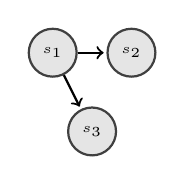
\begin{tikzpicture}[shorten >=1pt,->,scale=0.5]  
        \tikzstyle{sentence}=[circle,thick,draw=black!75,fill=black!10,minimum size=2mm]
        \tikzstyle{edge}=[draw, thick]
       \begin{scope}
         \node [sentence] (s1) at (0,2) {\tiny{$s_1$}};
         \node [sentence] (s2) at (2,2) {\tiny{$s_2$}};
         \node [sentence] (s3) at (1,0) {\tiny{$s_3$}}; 
         \path[edge] (s1) edge [above] node[font=\tiny] {} (s2);
         \path[edge] (s1) edge [above] node[font=\tiny] {} (s3);
        \end{scope}        
      \end{tikzpicture}
&
%%%%%%%%%%%%%%%%%%%%%%%%%%%%%% subgraph 2 %%%%%%%%%%%%%%%%%%%%%%%%%%%%%%
 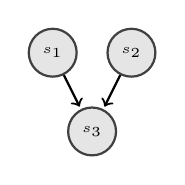
\begin{tikzpicture}[shorten >=1pt,->,scale=0.5]  
        \tikzstyle{sentence}=[circle,thick,draw=black!75,fill=black!10,minimum size=2mm]
        \tikzstyle{edge}=[draw, thick]
       \begin{scope}
         \node [sentence] (s1) at (0,2) {\tiny{$s_1$}};
         \node [sentence] (s2) at (2,2) {\tiny{$s_2$}};
         \node [sentence] (s3) at (1,0) {\tiny{$s_3$}}; 
         \path[edge] (s1) edge [above] node[font=\tiny] {} (s3);
         \path[edge] (s2) edge [above] node[font=\tiny] {} (s3);
        \end{scope}        
      \end{tikzpicture}

&
 %%%%%%%%%%%%%%%%%%%%%%%%%%%%%% subgraph 3 %%%%%%%%%%%%%%%%%%%%%%%%%%%%%%
 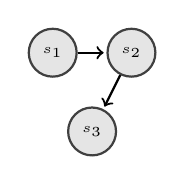
\begin{tikzpicture}[shorten >=1pt,->,scale=0.5]  
        \tikzstyle{sentence}=[circle,thick,draw=black!75,fill=black!10,minimum size=2mm]
        \tikzstyle{edge}=[draw, thick]
       \begin{scope}
         \node [sentence] (s1) at (0,2) {\tiny{$s_1$}};
         \node [sentence] (s2) at (2,2) {\tiny{$s_2$}};
         \node [sentence] (s3) at (1,0) {\tiny{$s_3$}}; 
         \path[edge] (s1) edge [above] node[font=\tiny] {} (s2);
         \path[edge] (s2) edge [above] node[font=\tiny] {} (s3);
        \end{scope}        
      \end{tikzpicture}
      
      
 &
 %%%%%%%%%%%%%%%%%%%%%%%%%%%%%% subgraph 7 %%%%%%%%%%%%%%%%%%%%%%%%%%%%%%
 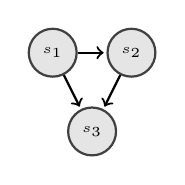
\begin{tikzpicture}[shorten >=1pt,->,scale=0.5]  
        \tikzstyle{sentence}=[circle,thick,draw=black!75,fill=black!10,minimum size=2mm]
        \tikzstyle{edge}=[draw, thick]
       \begin{scope}
        \node [sentence] (s1) at (0,2) {\tiny{$s_1$}};
         \node [sentence] (s2) at (2,2) {\tiny{$s_2$}};
         \node [sentence] (s3) at (1,0) {\tiny{$s_3$}}; 

         
         \path[edge] (s1) edge [above] node[font=\tiny] {} (s2);
         \path[edge] (s1) edge [above] node[font=\tiny] {} (s3);
         \path[edge] (s2) edge [above] node[font=\tiny] {} (s3);
         
        \end{scope}        
      \end{tikzpicture} 
\\

\scriptsize{$sg_1$} & \scriptsize{$sg_2$} & \scriptsize{$sg_3$}& \scriptsize{$sg_4$}
                 

\end{tabular}
}
\caption{Feasible 3\--node subgraph coherence features.}
\label{f:feasible_3node_subgraphs}
\end{figure}